\chapter{Estado del Arte}
\label{cap:EstadoArte}

\setlength{\parindent}{0pt}

En este capítulo se explicará que es blockchain, como funciona, que tipos hay, así como ver su uso en el presente y que aplicaciones se están desarrollando alrededor de la misma para sacarle su máximo potencial, este apartado es de crucial importancia pues servirá para ver el estado del arte de las aplicaciones (en concreto aplicaciones móvil) del presente.

% -------------------------------------------------- %
% -------------------------------------------------- %
\section{Blockchain}
Blockchain\cite{b1,b2,b3} es un término escuchado hoy en día por todas partes, más a nivel económico que tecnológico. Y aunque pueda parecer complejo, su funcionamiento es bastante sencillo.

% -------------------------------------------------- %
\subsection{Definición}
Blockchain es un tipo de base de datos, una base de datos es una colección de información guardada en un ordenador o servidor. Por norma general, la información esta guardada de forma ordenada y estructurada para poder ser accedida con comodidad. Las bases de datos no tienen un tamaño fijo, pudiendo crecer a niveles inimaginables, por norma general solo personal autorizado puede acceder a la información que se encuentra en ellas, así como añadir, eliminar y modificarla. \\

Entonces, ¿donde difiere la blockchain con una base de datos tradicional? \\

Una de las principales diferencias esta en el modo en el que se guarda la información, blockchain junta la información en grupos conocidos como \textbf{bloques}. Estos bloques tienen capacidad para una cantidad de información, y una vez llenos se enlazan con el bloque anterior con la ayuda de un \textbf{hash}. Un \textbf{hash}\cite{whatIsHash} es un algoritmo que mezcla la información que se le introduce para generar una salida única e irreversible de siempre la misma longitud. \\

\begin{figure}[h!]
  \centering
  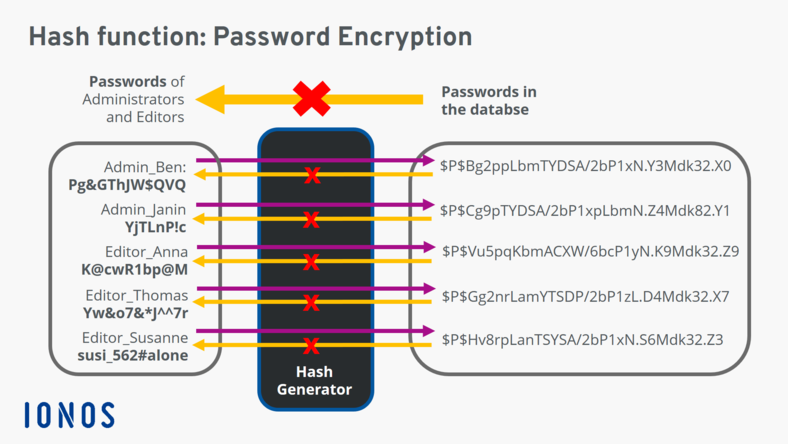
\includegraphics[width=0.6\linewidth]{figs/EstadoArte/Blockchain/hash}
  \caption[Hash]{Ejemplo genérico del funcionamiendo de un algorítmo hash}
  \label{fig:hash}
\end{figure}

\clearpage

Existen múltiples algorítmos hash, y van evolucionando con el tiempo siendo cada vez más seguros y con menos colisiones. Una colisión, se da cuando dos entradas diferentes producen el mismo resultado (rompiendo con una de las reglas principales de los algorítmos hash). \\

Para continuar con la explicación, utilizaremos como ejemplo la red de \textbf{Bitcoin}\cite{whatIsBitcoin} y su algorítmo de consenso \textbf{Proof of Work}\cite{whatIsProofOfWork}. La base es la misma para la inmensa mayoría de redes, sin embargo según el algorítmo de consenso el método difiere ligeramente. Los algorítmos se verán mas adelante. 

\begin{figure}[h!]
  \centering
  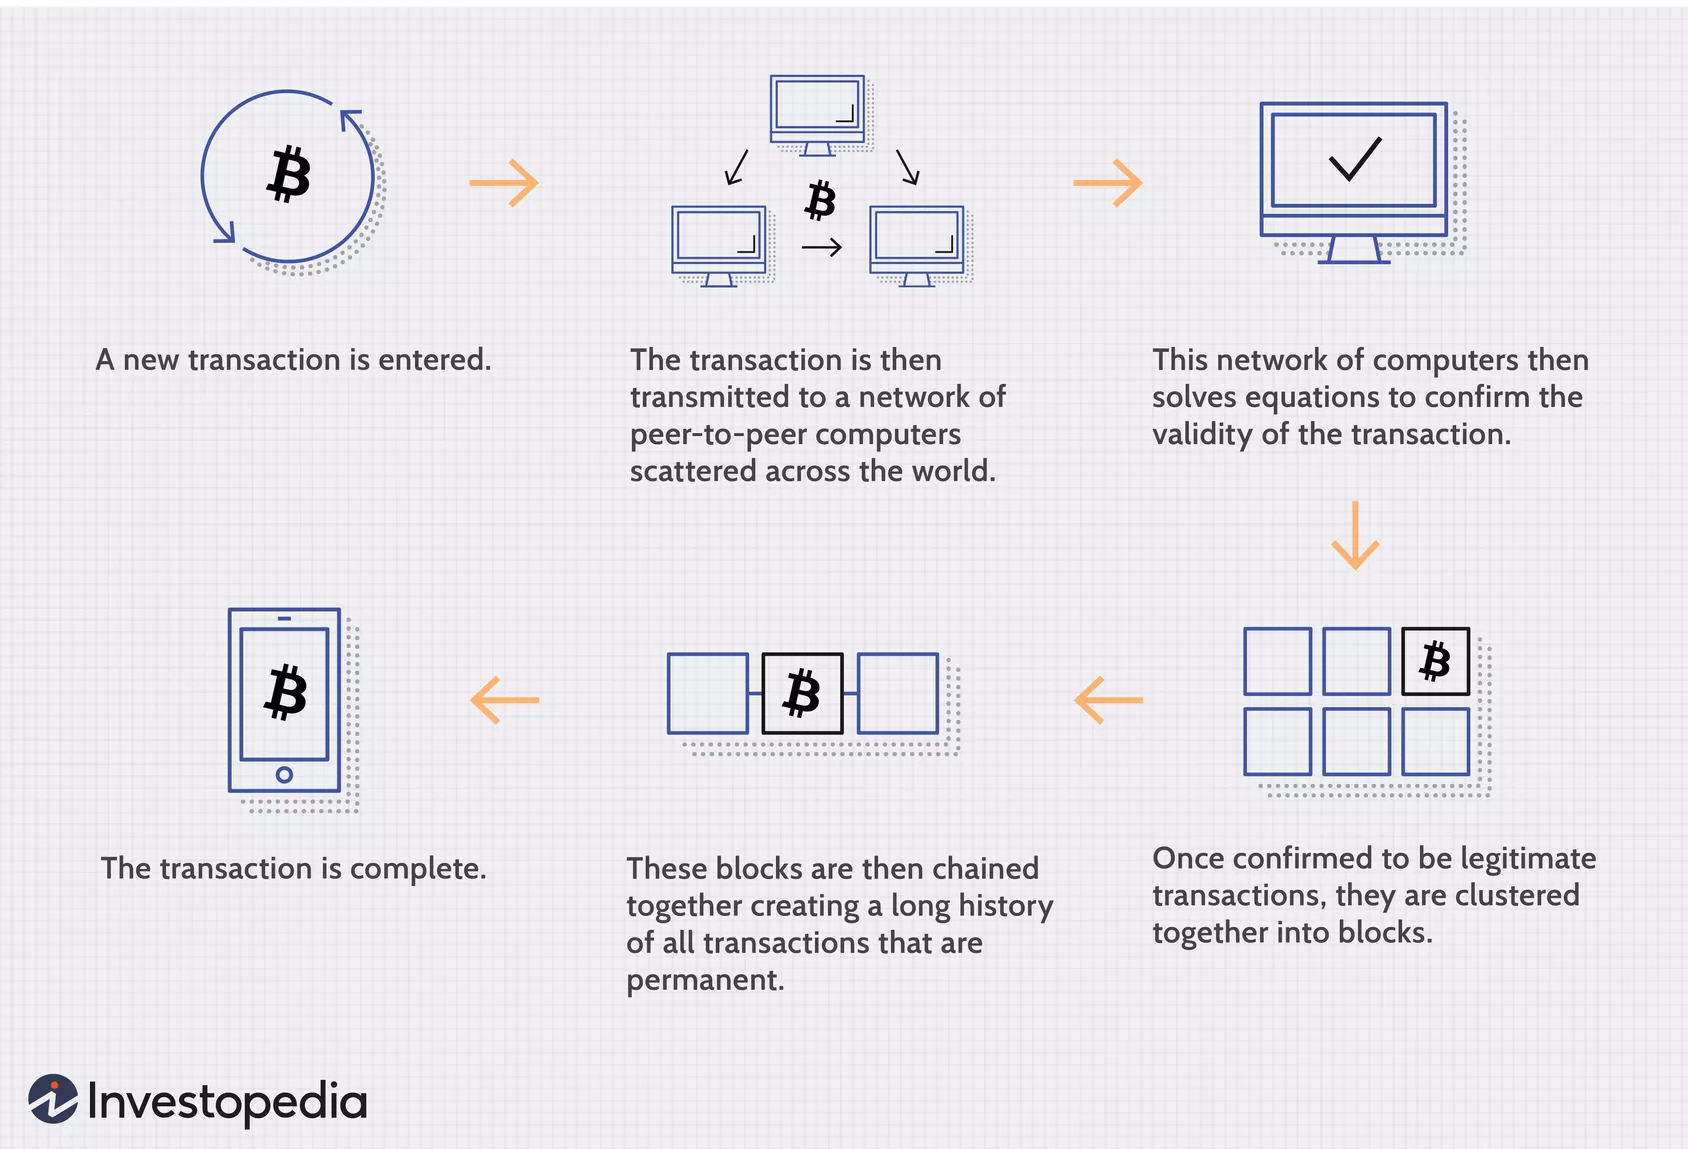
\includegraphics[width=0.8\linewidth]{figs/EstadoArte/Blockchain/bitcoinMining}
  \caption[Bitcoin Mining]{Transaction Process}
  \label{fig:bitcoin}
\end{figure}

Cada bloque de la blockchain, una vez tiene la cantidad de información necesaria para formar un bloque, pasa por una función \textbf{hash256}. Esta información es conocida como ``transacciones'', no son más que datos, ya sean monetarios, envio de datos (nombres, lugares, compras, firmas...) o cualquier tipo de información digital. Todos los nodos de la red comparten estas transacciones, estan todos sincronizados. Él hash por el que pasa la información tiene una especialidad, pues para evitar colisiones entre múltiples nodos de la blockchain, entendemos como nodo un ordenador de la red blockchain, y así evitar que varios bloques se quieran añadir simultaneamente, el hash resultante ha de tener una cantidad determinada de \verb|0|'s al principio del mismo. Por ejemplo, si la dificultad del hash es de \verb|32bits| la función hash256 resultante se puede ver así: \verb|000000003d3a75526946a3bcf00daec9fc9c9c4d51ddc7cc5df888f74dd434d1|. Para llegar a este hash, los nodos de la blockchain tienen que utilizar el hash del bloque anterior junto con la información de las transacciones, y junto con un número conocido como \textbf{nonce}\cite{whatIsNonce}. Un \textbf{nonce} es un número que solo puede ser usado una vez. Los nodos solo pueden modificar este número, no pueden tocar ni el hash del bloque anterior ni las transacciones. Los nodos proceden entonces a modificar de manera aleatoria este nonce hasta dar con el hash con los \verb|0|'s que se piden. Este procedimiento es completamente aleatorio, por lo que a más poder de computo, mas rápido puedes probar números y mas posibilidades tienes de dar con el hash que se pide. A este proceso se le llama ``minado''\cite{minarBitcoin}

\begin{figure}[h!]
  \centering
  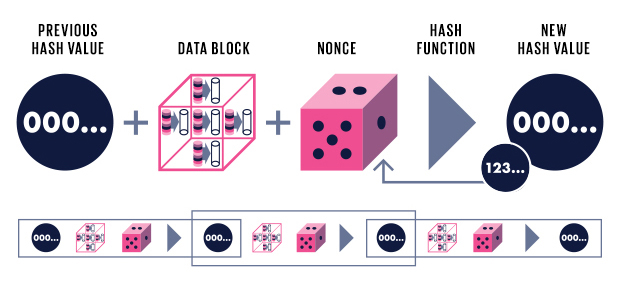
\includegraphics[width=0.8\linewidth]{figs/EstadoArte/Blockchain/hashDificultad}
  \caption[Hash dificultad]{Dificultad del hash}
  \label{fig:hashDiff}
\end{figure}

Una vez un nodo encuentra el nonce correto, lo comparte con el resto de nodos de la red blockchain los cuales validan la información, y se procede a añadir el nuevo bloque a la red blockchain. El nodo que ha encontrado el resultado correcto recibe un incentivo, en el caso de bitcoin, el nodo se asigna a si mismo un número de bitcoins, creando así nuevo bitcoin. 

% -------------------------------------------------- %
\subsection{Tipos de redes blockchain}

Cuando se habla de blockchain, parece dar la impresión de que solo existe un tipo. Sin embargo hay varias redes con sus ventajas y desventajas\cite{tiposBlock1}\cite{tiposBlock2}. Las principales diferencias entre ellas son las \textbf{funcionalidades, protocolos de consenso, administración y reglas para validar las transacciones}.

\subsubsection{Blockchain pública}

Las blockchain públicas no tienen permisos, cualquier usuario es bienvenido a unirse a la red, a enviar transacciones, a utilizar las funcionalidades que tiene la red, y a minar bloques. Las principales características de esta red son:
\begin{itemize}
\item Son \textbf{transparentes}: El código, el funcionamiento interno, los smart contracts si tiene (se verá este término mas adelante) son todos públicos y de código abierto.
\item \textbf{Sin permisos}: Cualquier persona puede unirse a la red sin preguntar. Lo único que tiene que hacer es descargar la red y sincronizarse con los demas nodos.
\item Usuarios \textbf{anónimos} y \textbf{sin administriador}: Nadie se conoce en la red, se trabaja siempre con lo que se conoce como \textbf{address}, que viene a ser un identificador único por miembro de la red para identificarlo. Además, no existe administrador de la red, no hay una persona o grupo que tenga poder sobre la red para hacer cambios de ningún tipo.
\item La información de la red puede ser \textbf{mantenida por todas las personas que lo deseen}. Y al minar nuevos bloques, dependiendo de la red, se ofrece un \textbf{incentivo}.
\end{itemize}

En resumidas cuentas, una blockchain pública es \emph{descentralizada}, \emph{distribuida}, \emph{consensuada}, \emph{abierta} y \emph{segura}. Algunos ejemplos de redes públicas son bitcoin\cite{webBitcoin} y ethereum\cite{webEthereum}

\subsubsection{Blockchain privada}

Las blockchains privadas son permisionadas, esto quiere decir que no cualquier persona puede añadirse como nodo libremente. Requieren de una \textbf{entidad} que ejerza de \textbf{administrador}. La mayoría de usuarios no consideran estas redes como blockchain a causa de esto. El administrador de la red tiene que dar permiso a los usuarios para poder minar, enviar transacciones y participar en general en la red. \\

Admeás, es abitual que los datos esten almacenados en servidores centrales y no abiertos al público. Pudiendo acceder a los bloques de la red solo mediante invitación. \\

Algunos ejemplos de blockchains privadas son R3\cite{webR3}, Ripple\cite{webRipple} y Quorum\cite{webQuorum}

\subsubsection{Blockchain híbrida o federada}

Estas redes son utilizadas por grandes empresas y gobiernos, no estan abiertas al público, teniendo la gestión varias entidades. Además no tienen una criptomoneda asociada y no recompensan por el minado de bloques. Sin embargo el software que utilizan es de código abierto, como puede ser \textbf{Hyperldger, Corda}\cite{webHpyer, webCorda}. \\

Como ejemplo tenemos la \emph{Enterprise Ethereum Alliance}, en la que participan el Banco Santander y BBVA. Esta red utiliza la blockchain de Ethereum (pública), sin embargo tienen su propia plataforma privada.

\subsubsection{Blockchain as a Service}

Estas redes blockchain son controladas por un proveedor de servicios como puede ser \emph{Amazon}. Estos proveedores permiten utilizar redes blockchain en la nube, permitiendo a los desarrolladores aprovechar el potencial de las redes blockchain sin la necesidad de invertir en el computo que ello requiere.

% -------------------------------------------------- %
\subsection{Tipos de algoritmo de consenso}

\begin{figure}[h!]
  \centering
  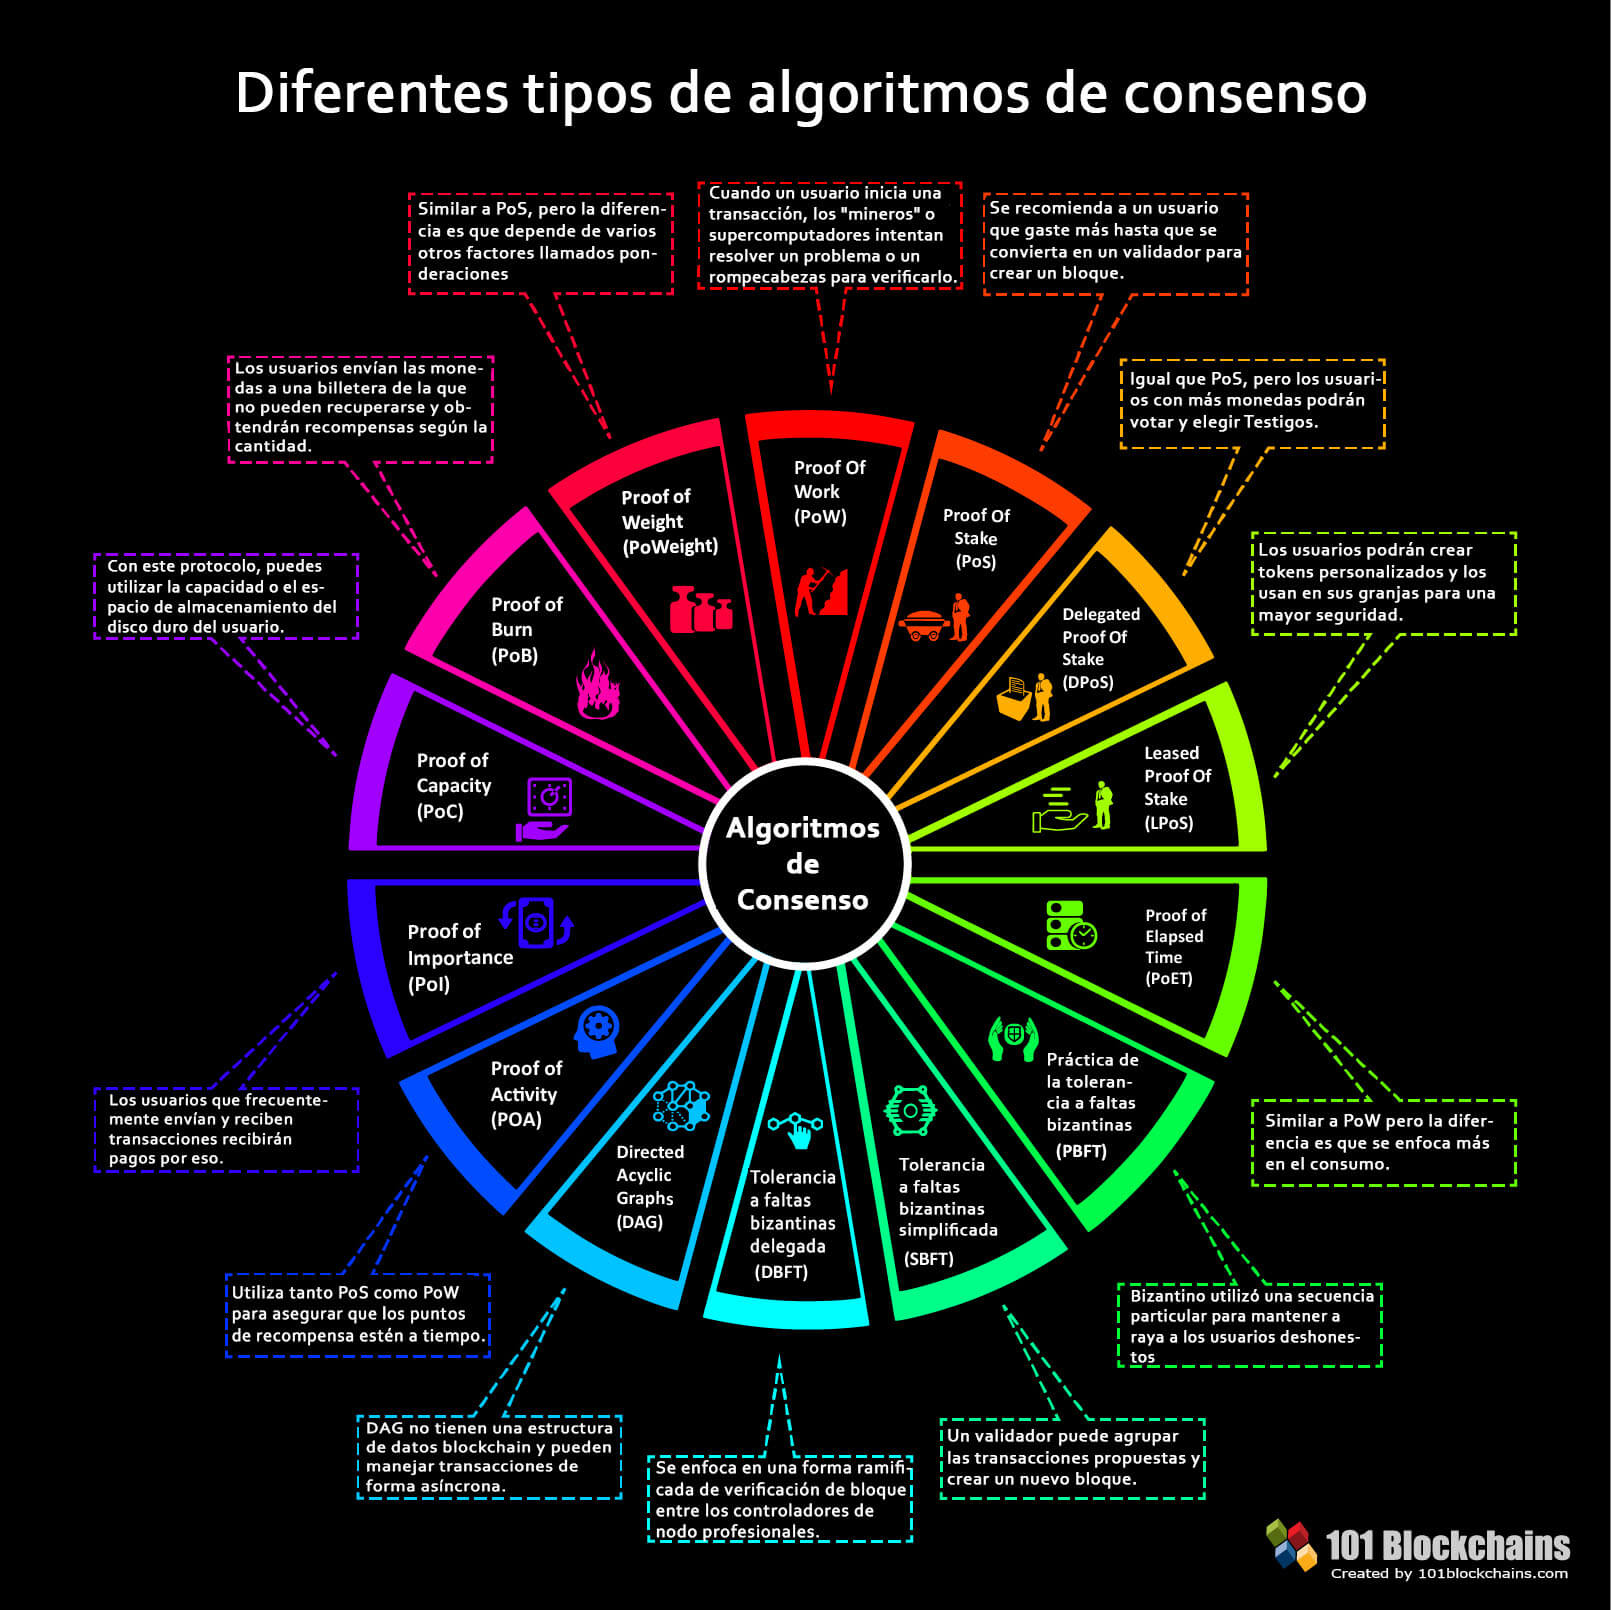
\includegraphics[width=0.8\linewidth]{figs/EstadoArte/Blockchain/algoritmosConsenso.jpeg}
  \caption[Algoritmos de Consenso]{Diferentes tipos de algoritmos}
  \label{fig:consenso}
\end{figure}

Existen múltiples algoritmos de consenso, y estos evolucionan con el paso del tiempo. Los algoritmos de consenso son procesos o protocolos de toma de decisiones, dependiendo del algoritmo hay uno o varios nodos de la red con el poder de tomar la decision sobre que bloque es el siguiente en añadirse a la red y si ha sido o no alterado. Los objetivos que busca blockchain con los algoritmos de consenso son:

\begin{itemize}
\item Llegar a un acuerdo
\item Cooperación
\item Colaboración
\item Igualdad de derechos
\item Participación
\item Actividad
\end{itemize}

Puesto que hay una gran cantidad de algoritmos trataremos de explicar algunos a continuación.\cite{algoConsenso}

\subsubsection{Proof of Work (PoW)}
\subsubsection{Proof of Stake (PoS)}
\subsubsection{Proof of Elapsed Time (PoET)}
\subsubsection{Practical Byzantine Fault Tolerance (PBFT)}
\subsubsection{Simplified BFT (SBFT)}


% -------------------------------------------------- %
\subsection{Smart contracts}


% -------------------------------------------------- %
\subsection{Usos en el presente}


% -------------------------------------------------- %
% -------------------------------------------------- %
\section{Proyectos Blockchain usando aplicaciones móvil}


% -------------------------------------------------- %
\subsection{App-1}


